\documentclass[aspectratio=169]{beamer}

\mode<presentation>
{
  \setbeamertemplate{background canvas}[square]
  \pgfdeclareimage[width=6em,interpolate=true]{dsailogo}{../dsai-logo}
  \pgfdeclareimage[width=6em,interpolate=true]{erasmuslogo}{../erasmus-logo}
  \titlegraphic{\pgfuseimage{dsailogo} \hspace{0.2in} \pgfuseimage{erasmuslogo}}
  %\usetheme{default}
  \usetheme{Madrid}
  \usecolortheme{rose}
  \usefonttheme[onlysmall]{structurebold}
}

\usepackage{pgf,pgfarrows,pgfnodes,pgfautomata,pgfheaps,pgfshade}
\usepackage{amsmath,amssymb}
\usepackage{graphics}
\usepackage{ragged2e}
%\usepackage[utf-8]{inputenc}
\usepackage{colortbl}
\usepackage[absolute,overlay]{textpos}
\setlength{\TPHorizModule}{30mm}
\setlength{\TPVertModule}{\TPHorizModule}
\textblockorigin{10mm}{10mm}
\usepackage[english]{babel}
\usepackage{listings}
\setbeamercovered{dynamic}

\AtBeginSection[]{
  \begin{frame}<beamer>
  \frametitle{Outline}
  \tableofcontents[currentsection]
  \end{frame}
}

\title[Computer Vision]{Computer Vision\\$N$-View Reconstruction}
\author{dsai.asia}
\institute[]{Asia Data Science and Artificial Intelligence Master's Program}
\date{}

% My math definitions

\renewcommand{\vec}[1]{\boldsymbol{#1}}
\newcommand{\mat}[1]{\mathtt{#1}}
\newcommand{\ten}[1]{\mathcal{#1}}
\newcommand{\crossmat}[1]{\begin{bmatrix} #1 \end{bmatrix}_{\times}}
\renewcommand{\null}[1]{{\cal N}(#1)}
\def\Rset{\mathbb{R}}
\def\Pset{\mathbb{P}}
\DeclareMathOperator*{\argmax}{argmax}
\DeclareMathOperator*{\argmin}{argmin}
\def\norm{\mbox{$\cal{N}$}}
\newcommand{\lse}{\mathfrak{se}}
\newcommand{\lsim}{\mathfrak{sim}}


\newcommand{\stereotype}[1]{\guillemotleft{{#1}}\guillemotright}

\newcommand{\myfig}[3]{\centerline{\includegraphics[width={#1}]{{#2}}}
    \centerline{\scriptsize #3}}

\begin{document}

%%%%%%%%%%%%%%%%%%%%%%%%%%%%%%%%%%%%%%%%%%%%%%%%%%%%%%%%%%%%
%%             CONTENTS START HERE

%\setbeamertemplate{navigation symbols}{}

\frame{\titlepage}

%--------------------------------------------------------------------
%\part<presentation>{Part name}
%
%\frame{\partpage}

\begin{frame}
\frametitle{Readings}

Readings for these lecture notes:
\begin{itemize}
\item[-] Hartley, R., and Zisserman, A. (2004), {\em Multiple View Geometry in
  Computer Vision}, Cambridge University Press, Chapters 18--19.
\item[-] Triggs, B., McLauchlan, P., Hartley, R., and Fitzgibbon,
  A. (1999), Bundle adjustment --- A modern synthesis, \textit{Vision
    Algorithms: Theory and Practice}, Springer-Verlag.
\item[-] Tomasi and Kanade, Sturm and Triggs, Pollefeys et al.,
  Davison et al., Klein and Murray, Lourakis and Argyros, Kerl, Sturm,
  and Cremers.
\end{itemize}

These notes contain material $\copyright$ Hartley and Zisserman
(2004) and others.

\end{frame}

%--------------------------------------------------------------------
\section{Introduction}
%--------------------------------------------------------------------

\begin{frame}
\frametitle{Introduction}
\framesubtitle{Reconstruction from $N$ views}

We have seen two-view projective and metric reconstruction techniques.
As we move to many views, however, what can we do?

\medskip

In this part we consider how to obtain a sparse
reconstruction given a \alert{sequence} of images.

\medskip

This is where Hartley and Zisserman's book becomes a little obsolete,
as there have been many new developments since 2004.

\end{frame}


\begin{frame}{Introduction}{History}

  A brief tour of the history:
  \begin{enumerate}
    \item 1970's: The term \alert{bundle adjustment} emerges in the
      photogrammetry literature, referring to simultaneous
      optimization of parameters of a set of cameras and a set of
      points observed by those cameras.
    \item 1992: Tomasi and Kanade show how to use SVD to factor the
      observation matrix to estimate a sequence of cameras and
      collection of 3D points.  Limited to affine cameras with no
      missing points.
    \item 1996: Sturm and Triggs show how to use iterative
      factorization to obtain a projective reconstruction. Other
      factorization methods refine the technique.
    \item 2004: Pollefeys et al.\ combine keyframe selection, SfM, BA,
      resectioning, loop closure, autocalibration, and 3D mesh
      techniques to obtain textured 3D models from videos obtained
      with hand-held cameras.
  \end{enumerate}

  Most offline 3D reconstruction methods use a pipeline similar to
  Pollefeys' approach, with manual intervention.

\end{frame}


\begin{frame}{Introduction}{History}

  More recently, SfM (computer vision) and SLAM (robotics) techniques
  are starting to converge.

  \begin{enumerate}
    \item 2006: Davison et al. introduce the first real-time monocular
      SLAM method, called \alert{MonoSLAM}.
    \item 2007: Klein and Murray introduce \alert{PTAM} (Parallel
      Tracking and Mapping) aimed at augmented realilty applications.
    \item 2009: Lourakis and Argyros introduce \alert{SBA} (Sparse
      BA), an efficient open source bundle adjustment library,
      bringing fast BA to the masses.
    \item 2013: Kerl, Sturm, and Cremers introduce \alert{DVO SLAM}
      (Dense Visual SLAM) for RBG-D cameras.
  \end{enumerate}

\end{frame}


\begin{frame}{Introduction}{History}

  As compute power increases, we are seeing
  more incremental real time methods with excellent results.
  
  \begin{enumerate}
      \item 2014: Engel, Sch\"{o}ps, and Cremers introduce \alert{SVO}, a
      semi-direct method for monocular visual odometry.
    \item 2014: Engel, St\"{u}ckler, and Cremers (2015) introduce LSD
      SLAM (Large-Scale Direct Monocular SLAM), the first dense
      monoSLAM method.
    \item 2015: Mur-Artal, Montiel, and Tard\'{o}s introduce ORB-SLAM,
      the most robust feature-based monoSLAM method today, combining
      the basic approach of PTAM with ORB features, BA, and loop
      closure techniques.
  \end{enumerate}

  LSD SLAM brings the idea of dense photometric alignment from RGBD to
  RGB, providing richer maps than ORB-SLAM at higher computational
  cost.

\end{frame}


\begin{frame}{Introduction}{History}

  Today, work is continuing on improving the robustness and efficiency
  of visual SLAM systems.

  \medskip

  Several methods now obtain real time results on smartphones or embedded
  platforms like the Odroid XU4 or NVidia TX2.

  \medskip

  However, it is still very difficult for state-of-the-art methods to
  keep track of a set of features during rotations and fast relative
  motion.

  \medskip

  \alert{Visual-inertial SLAM} systems attempt to combine IMU readings
  (linear acceleration and rotational velocity) with vision.

  \medskip

  Knowing approximately how the camera has moved since the last keyframe
  gives us a better idea of where to look for features in the next frame.

\end{frame}


\begin{frame}{Introduction}{History}

  Some visual-inertial SLAM systems:
  \begin{itemize}
    \item Christian Forster's Ph.D.\ thesis (2016) demonstrates combination of
      SVO with IMU preintegration to achieve very accurate VISLAM. No
      open source implementation.
    \item 2016: Forster, Zhang, Gassner, Welberger, and Scaramuzza
      introduce \alert{SVO-2}, a faster, more accurate version of
      SVO incorporating Forster's IMU priors. Implementation is commercial
      (no open source).
    \item Ra\'{u}l Mur-Artal, and Juan D. Tard\'{o}s (2017) introduce
      \alert{VI-ORB}, a visual-inertial version of ORB-SLAM using Forster's
      IMU preintegration. The authors did not
      release an open source version, but there is a community developed
      version on github.
    \item Stefan Leutenegger, Simon Lynen, Michael Bosse,
      Roland Siegwart and Paul Timothy Furgale (2015) introduce \alert{OKVIS},
      ``Keyframe-based visual–inertial odometry using nonlinear optimization.''
      Open-source version maintained by the author available on github.
  \end{itemize}

\end{frame}


\begin{frame}{Introduction}{History}

  Interesting project for this class: VI-ORB or OKVIS experiments on
  Pixhawk or Android...

\end{frame}

%--------------------------------------------------------------------
\section{Bundle adjustment}
%--------------------------------------------------------------------

\begin{frame}
\frametitle{Bundle adjustment}
\framesubtitle{The idea}

Given a set of unknown 3D points $\vec{X}_j$ viewed by a set of
cameras with unknown projection matrices $\mat{P}^i$ at image points
$\vec{x}_j^i$, we seek to find the camera matrices $\mat{P}^i$ and 3D
points $\vec{X}_j$ minimizing the reprojection error
\begin{equation*}
\min_{\hat{\mat{P}}^i,\hat{\vec{X}}_j} \sum_{ij} 
d(\hat{\mat{P}}^i\hat{\vec{X}}_j,\vec{x}^i_j)^2
\end{equation*}

\medskip

Iterative minimization of this cost function is called \alert{bundle
adjustment} because it involves adjusting the bundle of rays between
each camera center and the set of 3D points.

\medskip

As formulated above, we need outlier removal prior to nonlinear least
squares optimization. However, Triggs, McLauchlan, Hartley, and
Fitzgibbon (1999) argue for a formulation with a more general cost
function allowing robust estimation with the outliers included.

\end{frame}


\begin{frame}
\frametitle{Bundle adjustment}
\framesubtitle{Problems with bundle adjustment}

There are two big \alert{problems} with bundle adjustment:
\begin{itemize}
\item It needs a good \alert{starting point} to begin optimization.
\item There can be a \alert{large number of parameters} involved in
  the minimization.  For $n$ points viewed by $m$ cameras we have
  $3n+11m$ parameters.  This makes the matrices used by
  Levenberg-Marquardt prohibitively large.\footnote{Remember the
      linear system we have to solve on each iteration of LM?
\begin{equation*}
      \left[ \mat{J}_{\vec{f}}^T(\vec{P})\mat{J}_{\vec{f}}(\vec{P}) +
          \mu\mat{I} \right] \delta{\vec{P}} =
          -\mat{J}^T_{\vec{f}}(\vec{P})\vec{f}(\vec{P}).
\end{equation*}}

\end{itemize}

\end{frame}


\begin{frame}
\frametitle{Bundle adjustment}
\framesubtitle{Solutions to the problems with bundle adjustment}

Solutions of the first problem (the initial solution)
generally involve linear methods such as \alert{factorization}.

\medskip

Solutions to the second problem (large parameter matrix):
\begin{itemize}
\item Reduce $n$ and/or $m$, by using a subset of the points or
  partitioning the views [\alert{suboptimal}].
\item Interleave estimation of camera matrices with estimation of 3D
  points [guaranteed to converge but \alert{slow}].
\item Use a sparse minimization routine:
  \begin{itemize}
  \item Download the \texttt{sba} (sparse bundle adjustment) open
    source software from \url{http://www.ics.forth.gr/~lourakis/sba/}
  \item (For Debian) install the \texttt{liblapack-dev} package,
    and add \texttt{-llapack} to your \texttt{gcc} command line.
  \item Call \texttt{sba\_motstr\_levmar()} to estimate motion
    ($\mat{P}_i$'s) and structure ($\mat{X}$).
  \end{itemize}
\end{itemize}

\end{frame}


%--------------------------------------------------------------------
\section{Factorization}
%--------------------------------------------------------------------

\begin{frame}
\frametitle{Factorization}
\framesubtitle{Affine factorization}

Tomasi and Kanade's algorithm is a maximum likelihood reconstruction
in the case of \alert{affine} cameras.

\medskip

It requires that \alert{all points} be seen in \alert{all views}.

\medskip

For affine cameras we write $\vec{x}=(x,y)^T$ and
$\vec{X}=(X,Y,Z)^T$.  Then we have the projection equation
\begin{equation*}
\vec{x} = \mat{M} \vec{X} + \vec{t}
\end{equation*}

We seek cameras $\{\mat{M}^i,\vec{t}^i\}$ and 3D points $\vec{X}_j$
such that the distance between estimated and predicted image points is
minimized:
\begin{equation*}
\min_{\mat{M}^i,\vec{t}^i,\vec{X}_j}
\sum_{ij}(\vec{x}_j^i-\hat{\vec{x}}_j^i)^2 =
\min_{\mat{M}^i,\vec{t}^i,\vec{X}_j}
\sum_{ij}\left(\vec{x}_j^i-(\mat{M}^i\vec{X}_j+\vec{t}^i)\right)^2.
\end{equation*}

\end{frame}

\begin{frame}
\frametitle{Factorization}
\framesubtitle{Affine factorization}

If we choose the centroid of the points to be the origin of the
coordinate system, then we can estimate the \alert{translation
  vectors} $\vec{t}^i$ easily.

\medskip

Under affine projection, the origin of the coordinate system is
projected to $(0,0)^T$ in the image.  This means that $\vec{t}$ needs
to translate the projection of the origin to the mean of the observed
image points:
\begin{equation*}
\vec{t}^i = \frac{1}{n} \sum_j \vec{x}^i_j.
\end{equation*}

\medskip

To simplify the remaining calculations, we set $\vec{t}^i=\vec{0}$ and
adjust the points $\vec{x}_i^j$ accordingly.

\end{frame}

\begin{frame}
\frametitle{Factorization}
\framesubtitle{Affine factorization}

Now we arrange the adjusted image points in the $2m\times n$
\alert{measurement matrix}
\begin{equation*}
\mat{W}=\begin{bmatrix}
\vec{x}_1^1 & \vec{x}_2^1 & \cdots & \vec{x}_n^1 \\
\vec{x}_1^2 & \vec{x}_2^2 & \cdots & \vec{x}_n^2 \\
\hdots & \hdots & \ddots & \hdots \\
\vec{x}_1^m & \vec{x}_2^m & \cdots & \vec{x}_n^m
\end{bmatrix}.
\end{equation*}

\medskip

We want to find $\mat{M}^i$ and $\vec{X}_j$ such that
\begin{equation*}
\mat{W} = \begin{bmatrix} \mat{M}^1 \\ \mat{M}^2 \\ \hdots \\
\mat{M}^m \end{bmatrix} \begin{bmatrix} \vec{X}_1 & \vec{X}_2 & \cdots
\vec{X}_n \end{bmatrix}.
\end{equation*}

\end{frame}

\begin{frame}
\frametitle{Factorization}
\framesubtitle{Affine factorization}

Since $\mat{M}$ and $\mat{X}$ are rank 3, their product is rank 3.

\medskip

Since in general $\mat{W}$ will not be rank 3 due to measurement
noise, we replace it with the best possible reconstruction, the matrix
$\hat{\mat{W}}$ which is rank 3 and closest to $\mat{W}$ in Frobenius
norm.

\medskip

Such a matrix $\hat{\mat{W}}$ can be computed easily using the SVD
$\mat{U}\mat{D}\mat{V}^T=\mat{W}$ by truncating $\mat{U}$ and
$\mat{V}$ to three columns to get $\hat{\mat{U}}$ and $\hat{\mat{V}}$,
then truncating $\mat{D}$ to a $3\times 3$ matrix $\hat{\mat{D}}$,
then finally letting
$\hat{\mat{W}}=\hat{\mat{U}}\hat{\mat{D}}\hat{\mat{V}}^T$.

\medskip

Since $\hat{\mat{W}}$ minimizes $\|\mat{W}-\hat{\mat{W}}\|_F$,
$\hat{\mat{M}}=\hat{\mat{U}}$ and $\hat{\mat{X}}=\hat{\mat{V}}^T$ is a
maximum likelihood reconstruction.

\medskip

So we see that a straightforward application of the SVD gives us an
\alert{optimal reconstruction} in the case of \alert{affine cameras}.

\end{frame}

\begin{frame}
\frametitle{Factorization}
\framesubtitle{Projective factorization}

The affine factorization method doesn't work for \alert{projective
reconstruction}, so any serious projective distortion will introduce
error into the reconstruction.

\medskip

Sturm and Triggs (1996), however, pointed out that if we knew the
\alert{projective depth} of each point, then the structure and motion
(camera matrices) could be estimated correctly by factorization.

\medskip

We have $\vec{x}_j^i=\mat{P}^i\vec{X}_j$.  With a projective camera we have
homogeneous points and there is an implicit constant factor which we
can make explicit as $\lambda_j^i\vec{x}_j^i=\mat{P}^i\vec{X}_j$
with $\vec{x}_j^i=(x_j^i,y_j^i,1)^T$.

\end{frame}

\begin{frame}
\frametitle{Factorization}
\framesubtitle{Projective factorization}

If we write the depths explicitly and all points are visible in all
images, we can write the problem in terms of a \alert{scaled
measurement matrix}:
\begin{equation*}
\mat{W} =
\begin{bmatrix}
\lambda_1^1\vec{x}_1^1 & \lambda_2^1\vec{x}_2^1 & \cdots &
\lambda_n^1\vec{x}_n^1 \\
\lambda_1^2\vec{x}_1^2 & \lambda_2^2\vec{x}_2^2 & \cdots &
\lambda_n^2\vec{x}_n^2 \\
\vdots & \vdots & \ddots & \vdots \\
\lambda_1^m\vec{x}_1^m & \lambda_2^m\vec{x}_2^m & \cdots &
\lambda_n^m\vec{x}_n^m \end{bmatrix} =
\begin{bmatrix} \mat{P}^1 \\ \mat{P}^2 \\ \vdots \\ \mat{P}^m
\end{bmatrix} \begin{bmatrix} \vec{X}_1 & \vec{X}_2 & \cdots &
\vec{X}_n \end{bmatrix}
\end{equation*}

\medskip

Since $\mat{P}$ and $\mat{X}$ are each rank 4, $\mat{W}$ will be rank
4 and the \alert{rank 4 factorization} from the SVD will give a valid $\mat{P}$
and $\mat{X}$.

\end{frame}

\begin{frame}
\frametitle{Factorization}
\framesubtitle{Projective factorization}

The key to projective factorization is how to choose the
\alert{projective depths}\footnote{The $\lambda_j^i$ are called
projective depths because in a Euclidean frame they would be the
lengths of the projections of the scene points onto the cameras'
principal axes.}  $\lambda_j^i$?
\begin{itemize}
\item We could use another reconstruction method to estimate
  $\lambda_j^i$.
\item We can also initialize them arbitrarily, e.g.\ $\lambda_j^i=1$,
  then \alert{interleave} factorization with depth estimation.
\end{itemize}

\medskip

Though there is no guarantee that the iterative method will converge
to a global minimum, it is widely used in practice.

\end{frame}

\begin{frame}
\frametitle{Factorization}
\framesubtitle{Projective factorization}

The algorithm works well in practice, but it is important to
know \alert{what cost function} is it minimizing.

\medskip

By using rank 4 decomposition, it turns out the algorithm is
minimizing
\begin{equation*}
\|\mat{W}-\hat{\mat{W}}\|_F^2 =
\sum_{ij} \|\lambda_j^i\vec{x}_j^i - \hat{\lambda}_j^i\hat{\vec{x}}_j^i\|^2 =
\sum_{ij} (\lambda_j^ix_j^i - \hat{\lambda}_j^i\hat{x}_j^i)^2 +
          (\lambda_j^iy_j^i - \hat{\lambda}_j^i\hat{y}_j^i)^2 +
          (\lambda_j^i - \hat{\lambda}_j^i)^2
\end{equation*} 

When the $\lambda_j^i$ are close to each other, we see that the cost
function is an \alert{approximation to a scaled geometric distance}.

\end{frame}

\begin{frame}
\frametitle{Factorization}
\framesubtitle{Projective factorization}

Because the projective reconstruction cost function involves
$\lambda_j^i$, and the projective factorization method minimizes
geometric error when $\forall i,j, \lambda_j^i=1$, we would like to
keep the $\lambda_j^i$ \alert{as close to 1 as possible}.

\medskip

If we scale $\mat{P}$ and $\mat{X}$, we obtain
\begin{equation*}
(\alpha^i\beta_j\lambda_j^i)\vec{x}^i_j =
(\alpha^i\mat{P}^i)(\beta_j\vec{X}_j)
\end{equation*}
which means we can replace the projective depths by multiplying the
\alert{$i$th row} or \alert{$j$th column} of $\mat{W}$ by an
\alert{arbitrary factor}.

\medskip

One normalization method producing good results in practice is to
renormalize, on every iteration, the rows and columns of $\mat{W}$ so
they have \alert{unit norm}.

\medskip

As always, the \alert{image points} should be normalized by \alert{isotropic
scaling} before beginning.

\end{frame}

\begin{frame}
\frametitle{Factorization}
\framesubtitle{Projective factorization}

\begin{block}{Projective factorization: Objective}
Given a set of $n$ image points seen in $m$ views:
\begin{equation*}
\vec{x}_j^i ; i = 1, \ldots, m, \hspace{0.2in} j=1,\ldots,n
\end{equation*}
compute a projective reconstruction.
\end{block}

\end{frame}

\begin{frame}
\frametitle{Factorization}
\framesubtitle{Projective factorization}

\begin{block}{Projective factorization: Algorithm}
\begin{itemize}
\item[(i)] Normalize the image data using isotropic scaling.
\item[(ii)] Set projective depths $\lambda_j^i=1$ or use some other
  method to estimate them.
\item[(iii)] Normalize the depths $\lambda_j^i$ by multiplying rows
  and columns by constant factors.  One way is to do a pass setting the
  norm of each row to 1 then a pass setting the norm of each column to
  1.
\item[(iv)] Form the $3m\times n$ scaled measurement matrix $\mat{W}$
  and obtain $\mat{P}^i$ and $\mat{X}_j$ from the rank 4 factorization
  of $\mat{W}$.
\item[(v)] Reproject the points into each image to obtain new
  estimates of the depths and repeat from step (iii) until
  convergence.
\end{itemize}
\end{block}

\end{frame}


\begin{frame}
\frametitle{Factorization}
\framesubtitle{Factorization approaches to $N$-view reconstruction}

Factorization methods for reconstruction have received a great deal of
attention over the last 10 years.

\medskip

See Tang and Hung (2006) for a method based on the projective
factorization idea that \alert{allows missing points} and is also
\alert{guaranteed to converge} to a local minimum.

\end{frame}


%--------------------------------------------------------------------
\section{Resectioning}
%--------------------------------------------------------------------

\begin{frame}
\frametitle{Resectioning}
\framesubtitle{Motivation}

The factorization methods just outlined are \alert{batch} methods.

\medskip

They cannot be used to perform \alert{on-line} 3D estimation without
modification.

\medskip

The \alert{resectioning method} first gets an initial 3D
reconstruction using, for example, the SVD of $\mat{E}$, then repeats
the following steps for frame $i$:
\begin{itemize}
\item Get correspondences between already-estimated 3D points
  $\{\vec{X}_j\}_{j \in 1\ldots n}$ and new 2D points $\{\vec{x}_k\}_{k \in
    1\ldots m}$.
\item Use the correspondences to estimate $\mat{P}^i$.  This is called
  \alert{resectioning}.
\item Use triangulation to estimate new 3D points using
  correspondences between frame $i$ and frame $i-1$.
\end{itemize}

\end{frame}


\begin{frame}
\frametitle{Resectioning method}
\framesubtitle{Challenges in resectioning}

The main challenges in resectioning are \alert{accumulated error},
\alert{outliers}, and \alert{degenerate conditions}.

\medskip

To reduce accumulated error, we can periodically use bundle adjustment
to find a globally consistent, minimum error configuration of the
cameras and points.

\medskip

To mitigate the effect of outliers, we use RANSAC or other robust
estimators and outlier rejection.

\medskip

To avoid degenerate conditions, we apply \alert{keyframe selection},
in which we choose the images we use for reconstruction and
resectioning specifically to avoid degenerate configurations of the
cameras and points.

\medskip

This leads to the general algorithm, on the next page.

\end{frame}


\begin{frame}
\frametitle{Resectioning method}
\framesubtitle{The algorithm}

\begin{block}{Reconstruct from an image sequence: Algorithm II}
\begin{itemize}
\item[(i)] Compute \alert{interest points} in each image using, e.g.,
  SIFT.
\item[(ii)] Extract \alert{keyframes} from the image sequence
  in which significant motion separates successive keyframes.
\item[(iii)] Obtain 2-frame reconstruction from keyframes 1 and 2.
\item[(iv)] Perform \alert{resectioning} on remaining images.
\item[(v)] \alert{Bundle adjust} the cameras and 3D structure for the
  complete keyframe sequence to obtain a maximum likelihood projective
  reconstruction.
\end{itemize}
\end{block}

\end{frame}


\begin{frame}
\frametitle{Resectioning method}
\framesubtitle{Keyframe selection}

Keyframe selection \alert{improves the runtime performance} of 3D
reconstruction, helps improve \alert{accuracy}, and helps avoid
\alert{degeneracy}.

\medskip

Ahmed, Dailey, Landabaso, and Herrero (2010)\footnote{ Ahmed, M.T.,
  Dailey, M.N., Landabaso, J.L., and Herrero, N. (2010), Robust key
  frame extraction for 3D reconstruction from video streams.  In
  \textit{International Conference on Computer Vision Theory and
    Applications (VISAPP)}.} experimented with a variety of criteria
for robust key frame extraction.

\medskip

Given the first keyframe, we apply \alert{correspondence ratio} and
\alert{degeneracy avoidance} constraints to eliminate inappropriate
candidate keyframes.

\medskip

Then we select the best successor keyframe from the remaining
candidate keyframe set by maximizing an objective function.

\end{frame}


\begin{frame}
\frametitle{Resectioning method}
\framesubtitle{Keyframe selection}

The \alert{correspondence ratio} $R_{c}$ is a proxy for the baseline:
$$R_{c} = \frac{T_{c}}{T_{f}},$$
where $T_{c}$ is the number of inlier correspondences and $T_{f}$ is
total number of features found.

\medskip

Low values of $R_{c}$ indicate low overlap between two frames,
in turn indicating long baselines.

\medskip

Long baselines are desired for triangulation accuracy, but if the
number of corresponding points is insufficient, camera motion
estimation accuracy suffers.

\medskip

Thus, the correspondence ratio is constrained to lie between an upper
threshold $T_{1}$ and a lower threshold $T_{2}$.

\end{frame}


\begin{frame}
\frametitle{Resectioning method}
\framesubtitle{Keyframe selection}

To avoid degenerate cases, the \alert{geometric robust information criterion
(GRIC)} score is used to measure the goodness of fit for a homography
or the fundamental matrix.

$$GRIC = \sum_i \rho(e_{i}^{2}) + \lambda_{1}dn + \lambda_{2}k,$$
where $i = 1\ldots n$, $\rho(e_{i}^{2}) $ is a robust function
$$\rho(e_{i}^{2}) = min(\frac{e_{i}^{2}}{\sigma^2}, \lambda_{3}(r-d))$$
of the residual $e_i$ over the $n$ correspondences, $\sigma$ is the
assumed standard deviation of the error, $d$ is the model dimension, $k$ is
the model degrees of freedom, $r$ is the dimension of the data,
$\lambda_1 = log(r)$, $\lambda_2 = log(rn)$, and $\lambda_3$ limits
the residual error.

\medskip

The GRIC constraint is to \alert{reject} any candidate keyframes for
which the \alert{homography} model has a \alert{lower GRIC score} than
the \alert{fundamental matrix}.

\end{frame}


\begin{frame}
\frametitle{Resectioning method}
\framesubtitle{Keyframe selection}

After filtering by correspondence ratio and degeneracy constraints, we
select as the next keyframe the frame that maximizes certain selection
criteria incorporating
\begin{itemize}
\item \alert{Normalized GRIC difference}:
  $$f_{G}(i,j) = \dfrac{GRIC_{H}(i,j) - GRIC_{F}(i,j)}{GRIC_{H}}.$$
  The difference is maximized when the fundamental matrix model is
  much better than the homography model.
\item \alert{Point-to-epipolar line cost (PELC)}:
  $$f_{GP}(i,j) = w_{G}f_{G}(i,j) + w_{P}(\sigma - PELC(i,j)),$$
  where $i$ is the current keyframe and $j$ is a candidate next
  keyframe.  PELC tends to be high when correspondences are not
  accurate.
\end{itemize}

\end{frame}


\begin{frame}
\frametitle{Resectioning method}
\framesubtitle{Resectioning}

The camera matrix $\mat{P}^i$ is computed from 3D-2D correspondences
and the DLT algorithm.

\medskip

In practice, 3D reconstruction using \alert{long} video sequence
suffers from \alert{accumulated error}. Some issues are:
\begin{itemize}
\item \alert{Matching existing 3D to 2D points} in an additional frame
  is not perfect. Sometimes, already-existing features are treated as
  new points. This arises when the camera moves back and forth or when
  a point becomes occluded and then visible again.
\item Resectioning is highly sensitive to \alert{outliers}. The camera
  estimate can be completely wrong if we estimate $\mat{P}^i$ in the
  presence of outliers.
\end{itemize}

\end{frame}


\begin{frame}
\frametitle{Resectioning method}
\framesubtitle{Example from AIT Vision and Graphics Lab}

Atima Tharatipyakul worked on solving these problems by finding 2D-3D
point pairs using multiple frames then using RANSAC in camera
estimation to discard 2D-3D correspondences
outliers.\footnote{Tharatipyakul, A,, \textit{3D Visualization from
    Video Sequence for Agricultural Field Inspection Robot}, Master's
  thesis, Asian Institute of Technology, 2011.}

\medskip

Next slide: example results from resectioning method in Atima's work,
with 5 keyframes selected from a sequence of images containing
pineapples.

\medskip

3 of the keyframes are shown, along with camera estimates, point cloud
estimates, and fruit ellipsoid estimates.

\end{frame}


\begin{frame}
\frametitle{Resectioning method}
\framesubtitle{Example from AIT Vision and Graphics Lab}

\centerline{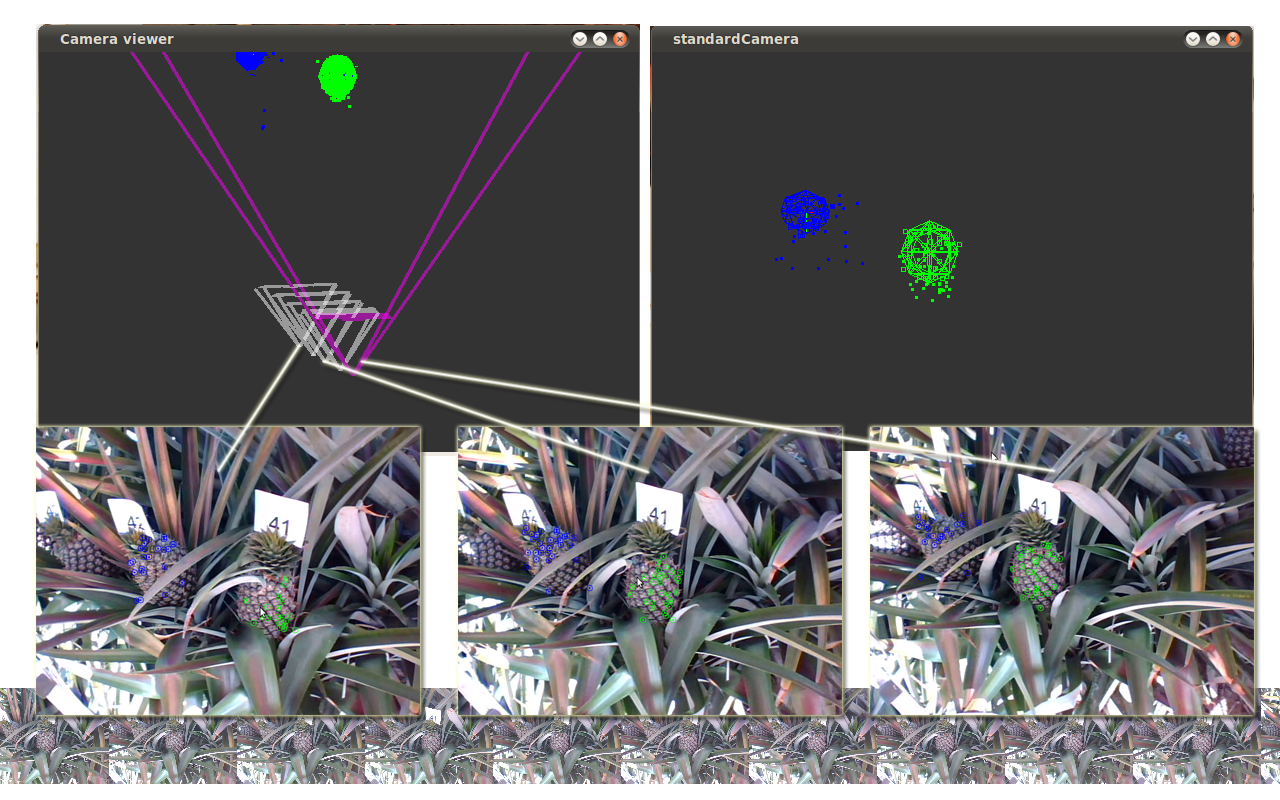
\includegraphics[width=4.5in]{3Doutput.png}}

\end{frame}


%--------------------------------------------------------------------
\section{Metric upgrade and auto-calibration}
%--------------------------------------------------------------------

\begin{frame}
\frametitle{Metric upgrade and auto-calibration}
\framesubtitle{Introduction}

As we already know, if $\mat{K}$ is known we can directly obtain
metric reconstructions. For two frames:
\begin{itemize}
\item For first pair of keyframes, estimate $\mat{F}$.
\item Calculate $\mat{E}$ from $\mat{F}$ and $\mat{K}$.
\item Factor $\mat{E}$ to obtain $\mat{P}'$ as described in H\&Z
  Section 9.6.
\end{itemize}

For $N$ frames, we factor $\mat{E}$ for the first pair of keyframes,
then use incremental resectioning and bundle adjustment.

\medskip

If $\mat{K}$ is \alert{unknown} or \alert{changing} during the image
sequence, however, we need a method for \alert{auto-calibration}.

\medskip

Here we look at some of the techniques for auto-calibration from
image correspondences over an image sequence.

\end{frame}


\begin{frame}
\frametitle{Metric upgrade and auto-calibration}
\framesubtitle{Idea of auto-calibration}

The idea of auto-calibration:
\begin{itemize}
\item Obtain a projective factorization $\mat{W}=\mat{P}\mat{X}$.
\item Estimate a homography $\mat{H}$ such that
  $\mat{W}=(\mat{P}\mat{H})(\mat{H}^{-1}\mat{X})$ is a metric
  reconstruction.
\item $\mat{P}^i\mat{H}$ is metric if it can be decomposed as
  $\mat{K}^i[\mat{R}^i \mid \vec{t}^i]$ where the $\mat{K}^i$
  are consistent with a priori constraints (the same across the
  image sequence, only focal length changing, etc.).
\end{itemize}

\end{frame}


\begin{frame}
\frametitle{Metric upgrade and auto-calibration}
\framesubtitle{Direct vs.\ stratified methods}

There are two main approaches to auto-calibration for general motion:
\begin{itemize}
\item \alert{Direct} estimation of $\mat{H}$.
\item \alert{Stratified} reconstruction, beginning with an affine
  reconstruction (which identifies $\vec{\pi}_{\infty}$) followed
  by metric reconstruction.
\end{itemize}

\medskip

Here we only consider direct methods, though stratified methods have
some advantages, mainly that there is a linear solution for
metric reconstruction once $\vec{\pi}_{\infty}$ is known (see text
for details).

\end{frame}


\begin{frame}
\frametitle{Metric upgrade and auto-calibration}
\framesubtitle{Framework}

We seek $\mat{H}$ such that $\mat{P}^i_M = \mat{P}^i\mat{H} =
\mat{K}^i[\mat{R}^i \mid \vec{t}^i]$ for $i = 1, \ldots, m$.

\medskip

Since we don't care about the absolute frame, we assume
$\mat{P}^1 = [ \mat{I} \mid \vec{0}]$ and that therefore $\mat{P}^1_M =
\mat{K}^1[\mat{I} \mid \vec{0}]$.

\medskip

In general, $\mat{H}$ takes the form
\begin{equation*}
\mat{H} = \begin{bmatrix} \mat{A} & \vec{t} \\ \vec{v}^T & k \end{bmatrix}.
\end{equation*}

\medskip

Since $\mat{P}^1_M = \mat{P}^1\mat{H} = [\mat{I} \mid \vec{0}]$, we can infer
that $\mat{A}=\mat{K}^1$ and $\vec{t}=\vec{0}$.

\medskip

Since $\mat{H}$ is necessarily non-singular we can assume $k=1$ to obtain
\begin{equation*}
\mat{H} = \begin{bmatrix} \mat{K}^1 & \vec{0} \\ \vec{v}^T & 1 \end{bmatrix}.
\end{equation*}

\end{frame}


\begin{frame}
\frametitle{Metric upgrade and auto-calibration}
\framesubtitle{Framework}

The plane at infinity $\vec{\pi}_{\infty}$ is $(0,0,0,1)^T$ in an affine
or metric
frame, and $\mat{H}^{-T}$ is the point/plane transform from the metric frame
to the projective frame.  This means we can derive
\begin{equation*}
\vec{\pi}_{\infty} =
\begin{pmatrix} -(\mat{K}^1)^{-T}\vec{v} \\ 1 \end{pmatrix}.
\end{equation*}

\medskip

Finally we can write
\begin{equation*}
\mat{H} =
\begin{bmatrix} \mat{K} & \vec{0} \\ -\vec{p}^T\mat{K} & 1 \end{bmatrix},
\vec{\pi}_{\infty} = (\vec{p}^T,1)^T.
\end{equation*}

\end{frame}

\begin{frame}
\frametitle{Metric upgrade and auto-calibration}
\framesubtitle{Framework}

For the rest of the cameras ($i = 2, \ldots, m$), we write
$\mat{P}^i = [\mat{A}^i \mid \vec{a}^i]$.

\medskip

Using $\mat{P}^i_M = \mat{P}^i\mat{H}$, we can obtain
    \begin{equation*}
    \mat{K}^i\mat{R}^i = (\mat{A}^i-\vec{a}^i\vec{p}^T) \mat{K}^1
    \end{equation*}
and (since $\mat{R}^i$ is orthogonal),
    \begin{equation*}
    \mat{K}^i\mat{K}^{iT} = (\mat{A}^i-\vec{a}^i\vec{p}^T)
           \mat{K}^1\mat{K}^{1T}(\mat{A}^i-\vec{a}^i\vec{p}^T)^T.
    \end{equation*}
These are the \alert{basic auto-calibration equations}.  If we know
$\mat{K}^1$, $\vec{p}$, and $\mat{P}^i$, we can calculate $\mat{P}^i_M$.

\end{frame}


\begin{frame}
\frametitle{Metric upgrade and auto-calibration}
\framesubtitle{The DIAC and the absolute dual quadric}

The matrix $\mat{K}^i\mat{K}^{iT}$ is the \alert{dual image of the
    absolute conic (DIAC)} $\mat{\omega}^{*i}$.

\medskip

The DIAC is the projection of the \alert{absolute dual quadric}
$\mat{Q}_{\infty}^*$:
\begin{equation*}
\mat{K}^i\mat{K}^{iT} = 
\mat{\omega}^{*i} = \mat{P}^i\mat{Q}^*_{\infty}\mat{P}^{iT}
\end{equation*}

\medskip

If we know $\mat{Q}^*_{\infty}$, we can calculate $\mat{K}^i$ directly
(by Cholesky decomposition of $\mat{P}^i\mat{Q}^*_{\infty}\mat{P}^{iT}$.

\end{frame}


\begin{frame}
\frametitle{Metric upgrade and auto-calibration}
\framesubtitle{Framework}

Important facts:
\begin{itemize}
\item The \alert{absolute conic} $\mat{\Omega}_{\infty}$
  is a conic on $\vec{\pi}_{\infty}$ containing
  the intersection of all circles and spheres with $\vec{\pi}_{\infty}$.
\item The \alert{absolute dual quadric} $\mat{Q}_{\infty}^*$ is a rank
  3 dual quadric whose envelope is the set of
  planes tangent to $\mat{\Omega}_{\infty}$.
\item The absolute dual quadric is invariant under similarity transforms
  and is just diag(1,1,1,0) in a metric frame.
\item The absolute dual quadric's null space is $\vec{\pi}_{\infty}$.
\end{itemize}

\end{frame}


\begin{frame}
\frametitle{Metric upgrade and auto-calibration}
\framesubtitle{Auto-calibration based on $\mat{Q}_{\infty}^*$}

\begin{block}{Auto-calibration based on $\mat{Q}_{\infty}^*$: Objective}
Given a set of matched points across several views and constraints on
the calibration matrices $\mat{K}^i$, compute a metric reconstruction of the
points and cameras.
\end{block}

\end{frame}

\begin{frame}
\frametitle{Metric upgrade and auto-calibration}
\framesubtitle{Auto-calibration based on $\mat{Q}_{\infty}^*$}

\begin{block}{Auto-calibration based on $\mat{Q}_{\infty}^*$: Algorithm}
\begin{itemize}
\item[(i)] Compute a projective reconstruction from a set of views,
    resulting in cameras $\mat{P}^i$ and points $\mat{X}$.
\item[(ii)] Use $\mat{\omega}^{*i} = \mat{P}^i\mat{Q}^*_{\infty}\mat{P}^{iT}$
    along with constraints to estimate $\mat{Q}^*_{\infty}$.
\item[(iii)] Decompose $\mat{Q}^*_{\infty}$ as
    $\mat{H}\tilde{\mat{I}}\mat{H}^T$ where $\tilde{\mat{I}}=$diag(1,1,1,0).
\item[(iv)] Apply $\mat{H}^{-1}$ to $\mat{X}$ and $\mat{H}$ to
    $\mat{P}^i$ to obtain a metric reconstruction of the point and cameras.
\item[(v)] Use iterative least squares to improve the solution.
\end{itemize}

\end{block}

\end{frame}


\begin{frame}
\frametitle{Metric upgrade and auto-calibration}
\framesubtitle{Auto-calibration based on $\mat{Q}_{\infty}^*$}

As a nice example of linear constraints on $\mat{Q}_{\infty}^*$,
see Pollefeys et al.\ (2004), Visual modeling with a hand-held
camera, \textit{IJCV} 59(3).

\medskip

As a nice example of more sophisticated methods to enforce the
rank 3, positive semidefiniteness, and ``chirality'' contraints on
$\mat{Q}_{\infty}$, see Chandraker et al.\ (2007), Autocalibration
via rank-constrained estimation of the absolute dual quadric,
In \textit{Proceedings of CVPR}.

\end{frame}

\end{document}

